\documentclass{beamer}
% https://tex.stackexchange.com/questions/258892/formatting-r-chunks-when-using-knitr

% pacotes
% \usepackage{Sweave} % para usar o Sweave, oras
 % para chamar outros arquivos Rnw, conforme https://support.rstudio.com/hc/en-us/articles/200486298-Working-with
\usepackage[brazil]{babel} % sudo tlmgr install babel-brazil   % sudo tlmgr update --self  % sudo tlmgr install babel-portuges
\usepackage[utf8]{inputenc}
\usepackage{fancybox}
\usepackage{textpos}  % sudo tlmgr install textpos
\usepackage{hyperref}
\usepackage{tcolorbox} % para caixas coloridas  % sudo tlmgr install tcolorbox

% Blind footnotes
\newcommand\blfootnote[1]{%
  \begingroup
  \renewcommand\thefootnote{}\footnote{#1}%
  \addtocounter{footnote}{-1}%
  \endgroup
}

% configuração dos links
\hypersetup
{
colorlinks=true,
linkcolor=blue,
urlcolor=blue,
filecolor=blue,
linktoc=all,
}

% pasta de imagens
\graphicspath{{./img/}}

% conteúdo
\title{Modelagem Preditiva}
\author{Filipe J. Zabala}
\institute{\href{https://www.pucrs.br/politecnica/}{Escola Politécnica} \\
           \href{https://www.pucrs.br/}{PUCRS} \\
           \href{https://github.com/filipezabala/}{github.com/filipezabala}}
\date{2021-06-21}

\usetheme{Pittsburgh}
\usecolortheme{owl} % sudo tlmgr install beamercolorthemeowl

% logo
\addtobeamertemplate{frametitle}{}{%
\begin{textblock*}{10mm}(-.05\textwidth,-.85cm)

\includegraphics[width=2cm]{logo_politecnica.png}
\end{textblock*}}

\begin{document}
\frame{\titlepage}

\begin{frame}
    \frametitle{Sumário}
    \tableofcontents
\end{frame}

\section{Minibio}
\begin{frame}{\secname}
Filipe J. Zabala $\cdot$ \url{filipe.zabala@pucrs.br}
\vspace{1cm}
  \begin{itemize}
    \item 2000-2004 Bacharel em Estatística (IME-UFRGS)
    \item 2006-2009 Mestre em Estatística (IME-USP)
    \item 2007-2009 Analista do Banco Itaú S.A.
    \item 2009-$\hphantom{2021}$ Sócio da ZN Consultoria Estatística
    \item 2010-$\hphantom{2021}$ Professor da Escola Politécnica da PUCRS
  \end{itemize}
\end{frame}

\section{Sobre modelagem preditiva}
\begin{frame}{\secname}
    \begin{itemize}
    \item Do Latim \textit{praedicere}, anunciar antecipadamente
    \pause
    \item Métodos para predizer novos valores de $X$
      \begin{itemize}
      \item $X$: variável de interesse
      \item $\theta$: parâmetro associado a $X$
      \end{itemize}
    \pause
    \item \textit{As duas culturas} de Leo Breiman (2001):
      \begin{itemize}
      \item interpretar $\theta$ \textit{vs} predizer $X$
      \end{itemize}
    \pause
    \item Debabrata Basu (1982): \textit{Information is what information does. It changes opinion (about $\theta$).}
    \pause
    \item Bruno de Finetti (1974): \textit{Probability, like beauty, exists only in the mind.}
    \pause
    \item George Box (1979): \textit{All models are wrong but some are useful.}
    \end{itemize}
\end{frame}

\section{Inferência bayesiana}
\begin{frame}{\secname}
    \begin{itemize}
    \item Priori: opinião (sobre $\theta$) antes de observar os dados \[ \pi(\theta) \]
    \pause
    \item Verossimilhança: informação dos dados \[ L(X|\theta) \]
    \pause
    \item Posteriori: opinião (sobre $\theta$) depois de observar os dados \[ \pi(\theta|X) \]
    \end{itemize}
\end{frame}

\begin{frame}{\secname}
    \begin{itemize}
    \item `A posteriori de hoje é a priori de amanhã'
    \pause
    \item Independência condicional (em relação a $\theta$)
    \pause
    \item Operação bayesiana: calibrar a opinião à luz dos dados \[ \pi(\theta|X) = \frac{\pi(\theta) L(X|\theta)}{\int_{\theta} \pi(\theta) L(X|\theta) d\theta} \propto \pi(\theta) L(X|\theta) \]
    \pause
    \item Preditiva: distribuição de $X$ \[ Pr(X=x) = \int_{\theta} \pi(\theta) L(X|\theta) d\theta \]
    \pause
    \item A probabilidade de o próximo resultado da moeda ser `cara` \[ Pr(X_{n+1}=\textrm{cara}) = \frac{r+1}{n+2} \]
    \end{itemize}
\end{frame}

% \section{Inferência bayesiana}
\begin{frame}{\secname}
    \begin{itemize}
    \item Variáveis permutáveis: a ordem das observações é indiferente \[ Pr(X_1=x_1, \ldots, X_N=x_N) = Pr(X_{\pi(1)}=x_1, \ldots, X_{\pi(N)}=x_N)  \]
    \pause
    \item Teorema da representação de de Finetti (1931) \[ Pr(X_1=x_1, \ldots, X_N=x_N) = \int_{\theta} \theta^a (1-\theta)^b \mu(d\theta) \]
    \pause
    \item Flexibiliza a suposição de independência
    \pause
    \item Trata $\theta$ apenas como uma variável de integração
    \end{itemize}
\end{frame}

\section{Exemplos}
\begin{frame}{Exemplo 1: Atribuição autoral}
\begin{figure}
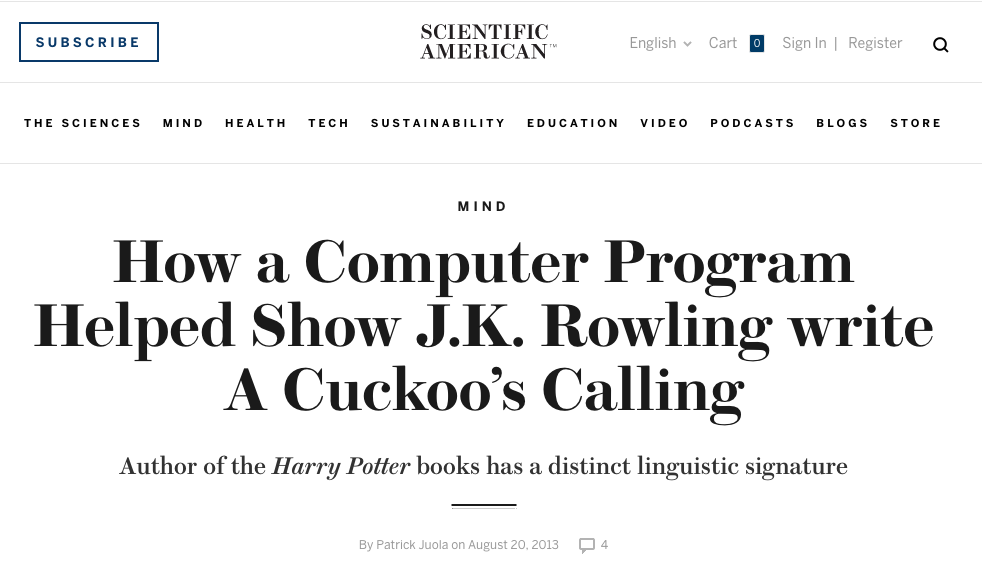
\includegraphics[scale=0.3]{jkrolling}
\end{figure}
\blfootnote{\tiny{\href{https://www.scientificamerican.com/article/how-a-computer-program-helped-show-jk-rowling-write-a-cuckoos-calling/}{Scientific American (2013-08-20) - How a Computer Program Helped Show J.K. Rowling write A Cuckoo’s Calling}}}
\end{frame}

\begin{frame}{Exemplo 1: Atribuição autoral}
\begin{figure}
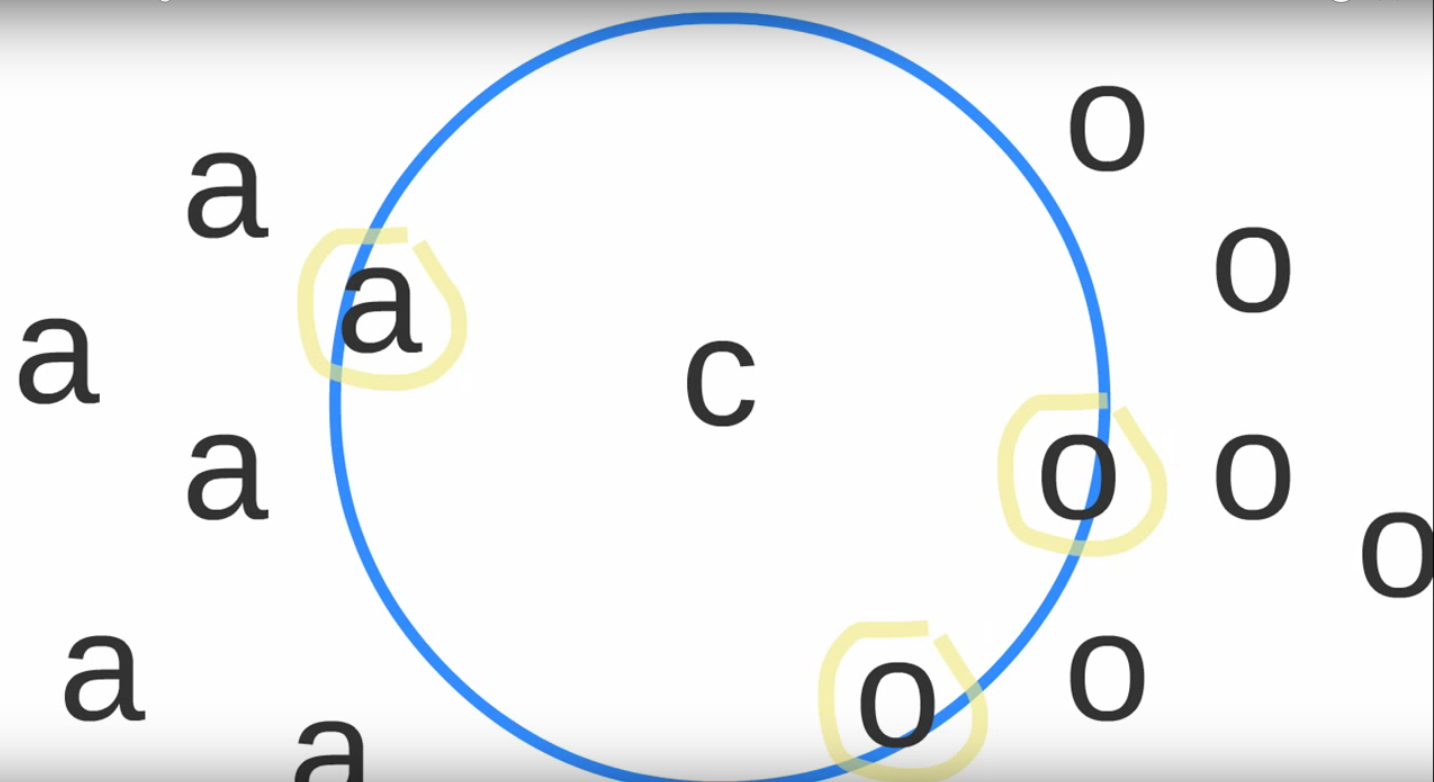
\includegraphics[scale=0.2]{knn}
\end{figure}
\blfootnote{\tiny{\href{https://www.youtube.com/watch?v=UqYde-LULfs}{Körting (2014) - How kNN algorithm works}}}
\end{frame}

\begin{frame}{Exemplo 2: Predição de séries temporais}
\begin{figure}
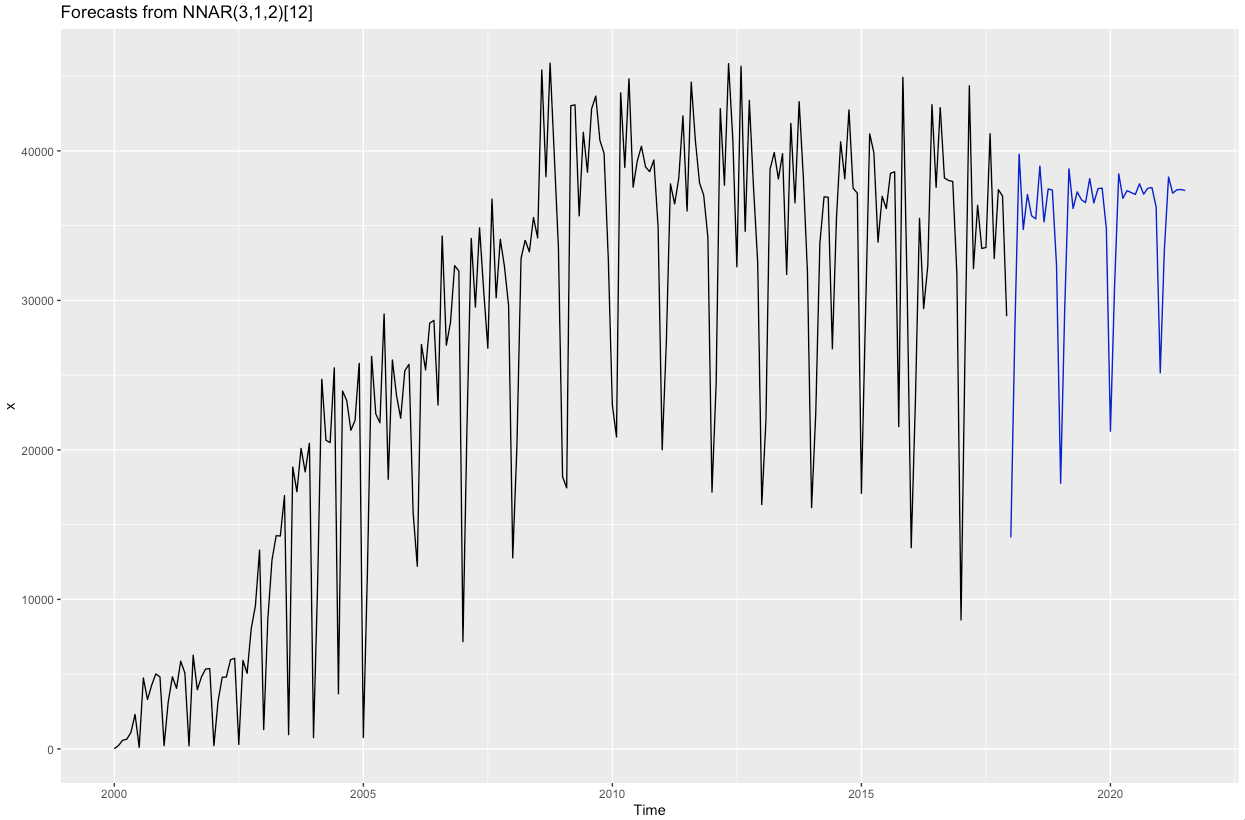
\includegraphics[scale=0.2]{forecast}
\end{figure}
\blfootnote{\tiny{\href{https://github.com/filipezabala/jurimetrics}{\nolinkurl{https://github.com/filipezabala/jurimetrics}}}}
\end{frame}

\begin{frame}{Exemplo 3: Classificação de falantes}
\begin{figure}
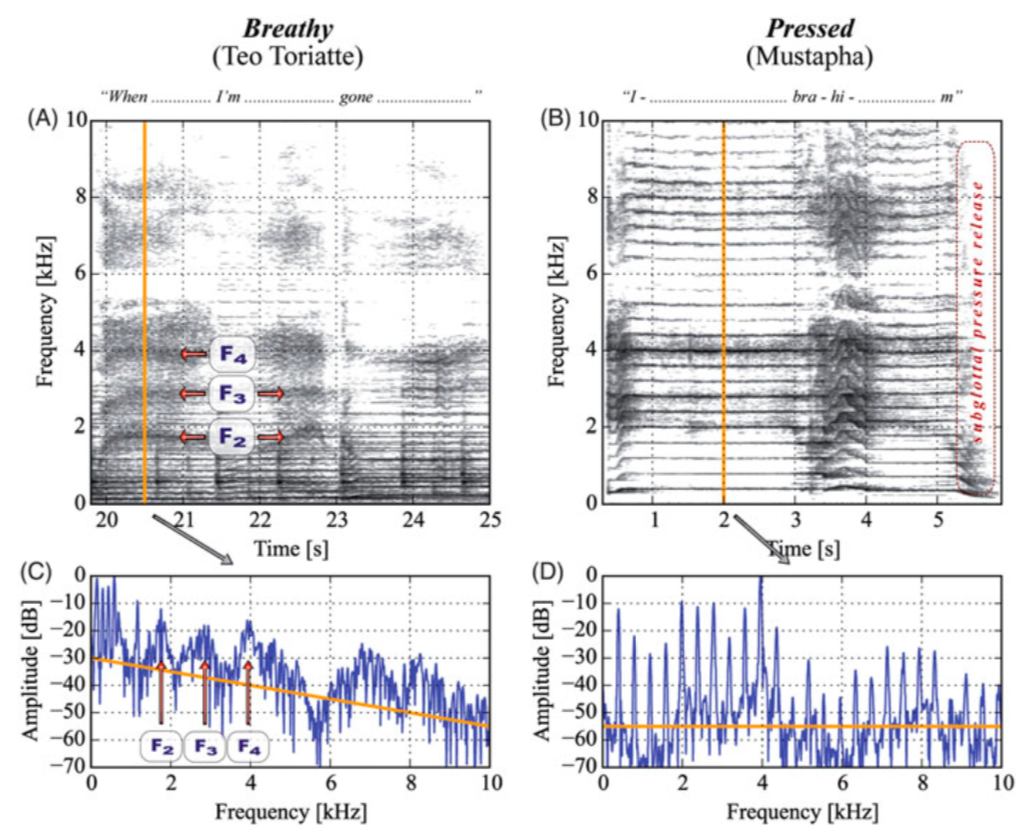
\includegraphics[scale=0.23]{freddie}
\end{figure}
\blfootnote{\tiny{\href{https://www.tandfonline.com/doi/abs/10.3109/14015439.2016.1156737}{Herbst et al (2016) - Freddie Mercury – Acoustic analysis of speaking fundamental frequency vibrato and subharmonics}}}
\end{frame}

\begin{frame}{Exemplo 4: Probabilidade de cenários eleitorais}
\begin{itemize}
\item Zabala (2009): O empate técnico é uma falácia
  \begin{itemize}
  \pause
  \item A metodologia dos institutos de pesquisa ignora que a soma dos percentuais deve ser 100\%
  \pause
  \item \href{http://www.filipezabala.com/cursos/dt.html}{Desempate técnico}
  \pause
  \item \href{http://www.pollingdata.com.br/}{Polling Data}
  \end{itemize}
\end{itemize}
\end{frame}

\begin{frame}{Exemplo 5: \textit{Gueule de bois}}
\blfootnote{\tiny{\href{https://www.artificiallawyer.com/2019/06/04/france-bans-judge-analytics-5-years-in-prison-for-rule-breakers/}{Artificial Lawyer (2019-06-04) - France Bans Judge Analytics, 5 Years In Prison For Rule Breakers}}}
\begin{figure}
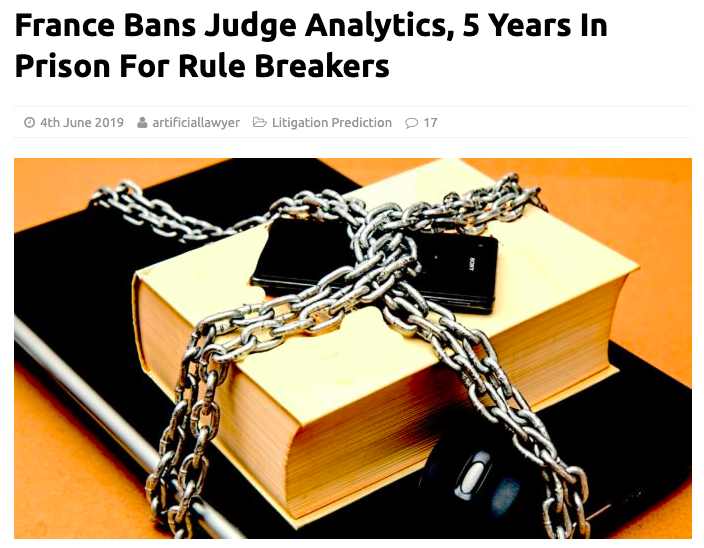
\includegraphics[scale=0.35]{franca}
\end{figure}
\end{frame}

\section{Para saber mais}
\begin{frame}{\secname}
    	\begin{itemize}
    	\item \href{https://doi.org/10.1017/CBO9780511569647}{Aitchison \& Dunsmore (1975) - Statistical Prediction Analysis}
    	\item \href{https://doi.org/10.1201/9780203742310}{Seymour Geisser (1993) - Predictive Inference - An Introduction}
    	\item \href{https://projecteuclid.org/euclid.ss/1009213726}{Breiman (2001) - Statistical Modeling: The Two Cultures}
    	\item \href{https://doi.org/10.11606/D.45.2009.tde-01032021-140004}{Zabala (2009) - Desempate Técnico}
    	\item \href{https://doi.org/10.1017/9781139236003}{Clarke \& Clarke (2018) - Predictive Statistics - Analysis and Inference Beyond Models}
    	\item \href{https://otexts.com/fpp2/}{Hyndman \& Athanasopoulos (2018) - Forecasting: Principles and Practice}
    	\item \href{http://www.rizbicki.ufscar.br/ame/}{Izbicki \& Santos (2020) - Aprendizado de Máquina: uma abordagem estatística}
	\end{itemize}
\end{frame}

\end{document}
